% =============================================================================
% formato/main.tex — Perfil de Proyecto de Grado
% Estructura según: Guía de Elaboración de Perfil Trabajos de Grado
% Universidad Privada del Valle — DAAP, 1ra Ed. 2019
%
% Motor requerido: XeLaTeX
%   Compilar con: latexmk -xelatex main.tex  (ejecutar desde esta carpeta)
%
% Dependencias:
%   univalle-perfil.cls  — enlace simbólico al directorio padre
%   ../imagenes/         — imágenes (logo en carátula, figuras del cuerpo)
%   ../referencias.bib   — base bibliográfica compartida
% =============================================================================

\documentclass{univalle-perfil}

\graphicspath{{../}}
\addbibresource{../referencias.bib}

\usepackage{tikz}
\usepackage{pgfplots}
\pgfplotsset{compat=newest}
\usetikzlibrary{shapes.geometric, positioning, arrows.meta}

% -----------------------------------------------------------------------------
% METADATOS DE LA CARÁTULA
% -----------------------------------------------------------------------------
\universidad{Universidad Privada del Valle}
\facultad{Facultad de Informática y Electrónica}
\carrera{Carrera de Licenciatura en Ingeniería de Sistemas}
\tituloTrabajo{Plataforma Web de Aprendizaje Adaptativo Basada en Grafos de Conocimiento para la Personalización del Estudio Autónomo de Matemáticas en Estudiantes del Colegio Cardenal Cushing en Santa Cruz de la Sierra}
\modalidad{Proyecto de Grado}
\tituloOptar{Licenciatura en Ingeniería de Sistemas}
\postulante{Franco Javier Torrez Alvarado}
\tutor{Rolando Lara Sanchez}
\ciudad{Santa Cruz}
\pais{Bolivia}
\anio{2026}

% =============================================================================
\begin{document}

% --- Carátula ----------------------------------------------------------------
\makecaratula

% --- Índices -----------------------------------------------------------------
\pagenumbering{gobble}
\tableofcontents
\listoffigures

% --- Contenido principal -----------------------------------------------------
\pagenumbering{arabic}

% =============================================================================
% 1. INTRODUCCIÓN
% =============================================================================
\section{Introducción}

El aprendizaje humano sigue un flujo de procesamiento de la información descrito por \textcite{atkinson1968}, que organiza la memoria en tres etapas: registro sensorial, memoria a corto plazo y memoria a largo plazo. Para que el conocimiento se consolide de manera real y duradera, la información debe atravesar cada etapa bajo condiciones específicas: atención sostenida, procesamiento activo y revisiones distribuidas en el tiempo.

Las plataformas educativas digitales existentes resuelven partes de este proceso de forma aislada. Khan Academy aplica rutas de aprendizaje sobre currículos predefinidos. Anki implementa repetición espaciada sin verificación de comprensión. Duolingo calibra la dificultad pero optimizando el engagement del usuario, no la retención profunda. Ninguna de estas plataformas integra todas estas soluciones en un sistema cohesivo, sin currículo fijo y adaptable a cualquier dominio de conocimiento.

En el contexto boliviano, el sistema educativo opera bajo un modelo estandarizado donde un solo docente atiende grupos de hasta treinta estudiantes, haciendo inviable la personalización del ritmo o del contenido. El acceso a tutorías privadas, que es la única alternativa de acompañamiento individualizado disponible hoy, tiene un costo que no está al alcance de todos los estudiantes.

El presente trabajo propone el desarrollo de una plataforma adaptativa de aprendizaje que organiza el conocimiento matemático de último año en un grafo de prerrequisitos, construye un modelo de usuario individual, implementa un motor de dificultad progresiva y un algoritmo de espaciado automático basado en la curva del olvido, y entrega retroalimentación inmediata después de cada ejercicio. El entregable principal es una arquitectura base funcional construida en fases incrementales, validada mediante pruebas técnicas y de usuario.

% =============================================================================
% 2. ANTECEDENTES DEL PROBLEMA
% =============================================================================
\section{Antecedentes del Problema}

Los estudiantes de último año del Colegio Cardenal Cushing en Santa Cruz de la Sierra estudian matemáticas de manera desordenada y pasiva, sin ninguna herramienta que organice los contenidos según su nivel individual, ajuste la dificultad de manera continua, verifique que la comprensión sea real antes de avanzar ni programe revisiones para evitar que los conceptos aprendidos se olviden. Este proceso genera conocimiento superficial, fragmentado y difícil de aplicar en la resolución de problemas.

El análisis del entorno de estudio actual se sintetiza en el Cuadro 2.1 mediante un análisis FODA, que identifica las fortalezas y debilidades del contexto actual, así como las oportunidades y amenazas que determinan el espacio de solución del problema.

\begin{table}[H]
\centering
\caption{Análisis FODA del entorno de estudio actual.}
{\renewcommand{\arraystretch}{1.5}
\begin{tabular}{|p{0.44\textwidth}|p{0.44\textwidth}|}
\hline
\textbf{Fortalezas} & \textbf{Oportunidades} \\
\hline
$\bullet$~Herramientas digitales de estudio disponibles globalmente (Anki, Khan Academy). \newline
$\bullet$~Algoritmos de repetición espaciada con fundamento científico comprobado. \newline
$\bullet$~Creciente acceso a dispositivos móviles e internet en Bolivia.
&
$\bullet$~Ausencia de soluciones integradas de aprendizaje adaptativo en el mercado boliviano. \newline
$\bullet$~Disponibilidad de modelos de lenguaje para generación automática de grafos de conocimiento. \newline
$\bullet$~Demanda creciente de herramientas de estudio independientes del currículo institucional.
\\
\hline
\textbf{Debilidades} & \textbf{Amenazas} \\
\hline
$\bullet$~Hábitos de estudio pasivos: relectura sin verificación de comprensión real. \newline
$\bullet$~Acceso a tutorías personalizadas limitado por costo. \newline
$\bullet$~Herramientas existentes operan sobre currículos fijos sin adaptación al usuario individual.
&
$\bullet$~Plataformas internacionales con mayores recursos podrían incorporar funcionalidades similares. \newline
$\bullet$~Dependencia de tecnologías de IA con evolución rápida y costos variables. \newline
$\bullet$~Resistencia al cambio de hábitos de estudio en estudiantes acostumbrados a métodos tradicionales.
\\
\hline
\end{tabular}}
\fuente{Elaboración propia, 2026.}
\end{table}

No existen en el mercado local plataformas que resuelvan de manera integrada el problema descrito. A nivel internacional, Khan Academy, Anki y Duolingo abordan partes del proceso de estudio de forma aislada, sin integrar grafos de conocimiento, espaciado automático y verificación de comprensión en un único sistema sin currículo fijo.

\subsection{Planteamiento del Problema}

Los estudiantes de último año del Colegio Cardenal Cushing en Santa Cruz de la Sierra presentan un proceso de estudio de matemáticas desorganizado y pasivo: no disponen de ninguna guía que organice los contenidos según sus conocimientos previos, ajuste la dificultad de manera continua, verifique que la comprensión sea real antes de avanzar ni programe revisiones para evitar que los conceptos se olviden, generando conocimiento superficial, fragmentado y difícil de aplicar en la resolución de problemas. ¿Cómo puede una plataforma web de aprendizaje adaptativo basada en grafos de conocimiento personalizar el estudio autónomo de matemáticas de los estudiantes del Colegio Cardenal Cushing, organizando los contenidos según su nivel individual, ajustando la dificultad de manera continua, verificando la comprensión real y programando revisiones automáticas para consolidar el conocimiento de forma eficiente?

\subsection{Objeto de Estudio}

El proceso de estudio autónomo de matemáticas de los estudiantes de último año del Colegio Cardenal Cushing en Santa Cruz de la Sierra: su organización de los contenidos, secuencia de estudio, nivel de comprensión alcanzado y retención de los conceptos matemáticos a lo largo del tiempo.

% =============================================================================
% 3. OBJETIVOS
% =============================================================================
\section{Objetivos}

\subsection{Objetivo General}

Desarrollar una plataforma web de aprendizaje adaptativo basada en grafos de conocimiento que personalice el estudio autónomo de matemáticas de los estudiantes de último año del Colegio Cardenal Cushing, mediante la organización de los contenidos matemáticos según sus prerrequisitos, el ajuste continuo de dificultad, la verificación de comprensión y la programación automática de repasos.

\subsection{Objetivos Específicos}

\begin{itemize}
    \item Analizar el proceso de estudio autónomo de matemáticas de los estudiantes del Colegio Cardenal Cushing mediante entrevistas y observación directa, para identificar los requerimientos funcionales y no funcionales de la plataforma.
    \item Diseñar la arquitectura de la plataforma web adaptativa, incluyendo el grafo de prerrequisitos del currículo de matemáticas de último año, el modelo de usuario, el motor de dificultad progresiva, el algoritmo de espaciado automático basado en la curva del olvido y el sistema de retroalimentación inmediata.
    \item Construir la plataforma mediante implementación incremental por módulos, integrando el grafo de conocimiento matemático, el modelo de usuario, el motor de dificultad, la verificación de comprensión, el algoritmo de espaciado y la retroalimentación.
    \item Evaluar el funcionamiento de la plataforma mediante pruebas funcionales basadas en los requerimientos definidos y pruebas de usabilidad con estudiantes del Colegio Cardenal Cushing, verificando que el sistema personaliza el estudio de matemáticas de manera efectiva.
\end{itemize}

% =============================================================================
% 4. JUSTIFICACIÓN
% =============================================================================
\section{Justificación}

El aprendizaje es una actividad que toda persona realiza de manera continua, pero los métodos y herramientas disponibles hoy no están diseñados para acompañar ese proceso de manera individual y eficiente. Este proyecto se justifica porque existe una brecha real entre cómo funciona la memoria humana y cómo está diseñado el entorno de estudio actual, y porque la tecnología disponible hoy permite cerrar esa brecha de una manera que antes no era posible.

\subsection{Justificación Técnica}

El proyecto es técnicamente viable porque cada uno de sus componentes tiene precedente en la industria. Los grafos de conocimiento, los algoritmos de espaciado basados en la curva del olvido y los modelos de usuario adaptativo son tecnologías maduras que ya existen por separado en plataformas como Anki, Khan Academy y Duolingo. Lo que no existe es un sistema que las integre de manera coherente aplicado específicamente al currículo de matemáticas de último año de colegio en Bolivia. El grafo de prerrequisitos matemáticos, el motor de dificultad progresiva y la retroalimentación inmediata son implementables con las herramientas de desarrollo disponibles actualmente. El entregable del proyecto es una arquitectura base funcional construida en fases incrementales, lo que hace el alcance técnico defendible dentro del tiempo de un proyecto de grado.

\subsection{Justificación Económica}

El costo anual de un estudiante en colegio privado en Santa Cruz de la Sierra, incluyendo mensualidades, útiles y transporte, oscila entre \$1.000 y \$1.200, sin ninguna garantía de que el proceso de estudio sea eficiente. El acceso a tutorías privadas, única alternativa de personalización disponible hoy, tiene un costo que no está al alcance de todos los estudiantes. El sistema propone un modelo de suscripción mensual que representa entre el 8\% y el 15\% del costo anual del colegio, con un costo marginal por usuario cercano a los \$0,15 mensuales en consumo de inteligencia artificial, lo que genera un margen sostenible desde etapas tempranas. A escala regional, el mercado de estudiantes de secundaria en Latinoamérica representa una oportunidad significativa para un sistema que no depende de ningún currículo institucional preestablecido.

\subsection{Justificación Social}

El sistema educativo actual genera una brecha entre los estudiantes que tienen acceso a acompañamiento personalizado y los que estudian solos, sin guía ni retroalimentación oportuna. Esta brecha se manifiesta en rendimiento académico y desarrollo de habilidades a largo plazo. Un sistema adaptativo accesible desde cualquier dispositivo, sin depender de un docente ni de un currículo institucional, democratiza el acceso a una experiencia de aprendizaje personalizada que hoy solo está disponible para quienes pueden pagar un tutor privado. El impacto social no se limita al colegio: el sistema es igualmente funcional para cualquier persona que quiera aprender algo por su cuenta, extendiendo su alcance más allá del entorno académico formal.

% =============================================================================
% 5. DELIMITACIÓN DE LA INVESTIGACIÓN
% =============================================================================
\section{Delimitación de la Investigación}

\subsection{Temática}

La investigación se delimita al desarrollo de una plataforma web de aprendizaje adaptativo orientada a personalizar el estudio autónomo de matemáticas de último año de colegio, mediante un grafo de prerrequisitos del currículo matemático, modelado del usuario, ajuste progresivo de dificultad, verificación de comprensión y programación automática de repasos. El proyecto no aborda otras materias del currículo escolar ni la evaluación pedagógica formal de largo plazo; se enfoca en el diseño, construcción y validación funcional de una solución de software aplicada al dominio de matemáticas.

\subsection{Espacial}

La investigación se desarrolla en la ciudad de Santa Cruz de la Sierra, Bolivia, tomando como población de referencia a estudiantes de último año de colegio. La validación inicial de la propuesta se realizará con estudiantes del Colegio Cardenal Cushing, debido al acceso disponible para aplicar entrevistas, pruebas de uso y observación del proceso de estudio. Aunque la plataforma puede adaptarse a otros contextos educativos, los resultados de esta investigación se interpretan dentro de este entorno específico.

\subsection{Temporal}

La investigación se desarrolla durante la gestión 2026, en el período comprendido entre abril y diciembre. En este intervalo se realiza el análisis del problema, diseño de la solución, desarrollo incremental de los módulos principales, integración del sistema y validación inicial con usuarios. Los resultados se limitan al estado de las tecnologías disponibles durante dicho período, especialmente en lo referente a modelos de lenguaje, generación automática de grafos de conocimiento y servicios de inteligencia artificial.

% =============================================================================
% 6. PROPUESTA DE SOLUCIÓN AL PLANTEAMIENTO DEL PROBLEMA
% =============================================================================
\section{Propuesta de Solución al Planteamiento del Problema}

El sistema propuesto es una plataforma adaptativa de aprendizaje que organiza los contenidos matemáticos de último año en un grafo de prerrequisitos del currículo, evalúa el nivel inicial del estudiante, genera una ruta de estudio personalizada, ajusta la dificultad de manera continua, verifica que la comprensión sea real antes de permitir el avance y programa revisiones automáticas para evitar el deterioro del conocimiento. El entregable principal del proyecto de grado es una arquitectura base funcional con los módulos centrales integrados y operativos, construida en fases incrementales y validada mediante pruebas técnicas y de usuario.

Los módulos centrales del sistema son los siguientes: el grafo de conocimiento dinámico, que organiza los conceptos y sus dependencias; el modelo de usuario individual, que registra el estado de cada concepto en tiempo real; el motor de dificultad progresiva, que calibra el nivel del contenido según el desempeño; el módulo de comprensión conectada, que verifica relaciones entre conceptos antes de permitir el avance; el algoritmo de espaciado automático, que programa revisiones en el momento óptimo; y el sistema de retroalimentación inmediata, que identifica y corrige fallas en tiempo real.

\begin{figure}[H]
\centering
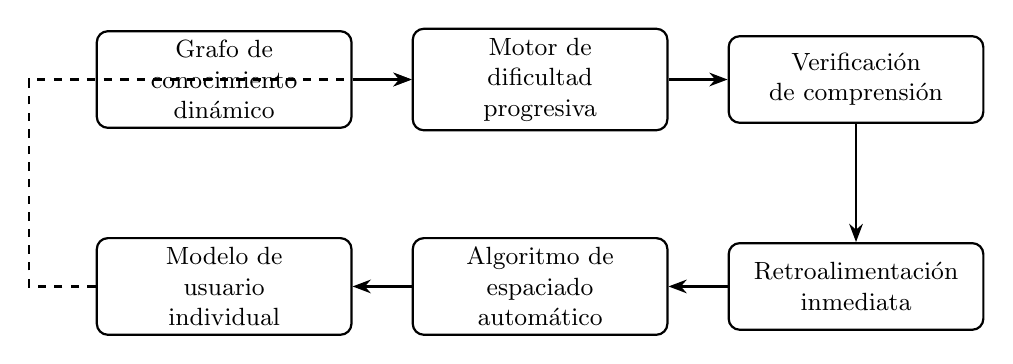
\begin{tikzpicture}[
  node distance=0.55cm and 0.75cm,
  box/.style={rectangle, rounded corners=4pt, draw, thick,
              text width=3.0cm, minimum height=1.1cm,
              align=center, font=\small},
  arr/.style={-{Stealth}, thick},
]
% Fila superior (izquierda a derecha)
\node[box] (grafo)  {Grafo de\\conocimiento\\dinámico};
\node[box, right=of grafo]  (motor)  {Motor de\\dificultad\\progresiva};
\node[box, right=of motor]  (verif)  {Verificación\\de comprensión};
% Fila inferior (derecha a izquierda, alineada debajo)
\node[box, below=1.5cm of verif]   (retro)     {Retroalimentación\\inmediata};
\node[box, left=of retro]           (espaciado) {Algoritmo de\\espaciado\\automático};
\node[box, left=of espaciado]       (usuario)   {Modelo de\\usuario\\individual};
% Flechas fila superior
\draw[arr] (grafo)      -- (motor);
\draw[arr] (motor)      -- (verif);
% Flecha columna derecha: abajo
\draw[arr] (verif.south) -- (retro.north);
% Flechas fila inferior
\draw[arr] (retro)      -- (espaciado);
\draw[arr] (espaciado)  -- (usuario);
% Retroalimentación: modelo de usuario actualiza el motor (lado izquierdo)
\draw[arr, dashed] (usuario.west) -- ++(-0.85,0) |- (motor.west);
\end{tikzpicture}
\caption{Módulos centrales de la plataforma y flujo de interacción entre componentes. La flecha punteada indica que el modelo de usuario retroalimenta continuamente al motor de dificultad.}
\fuente{Elaboración propia, 2026.}
\end{figure}

\begin{figure}[H]
\centering
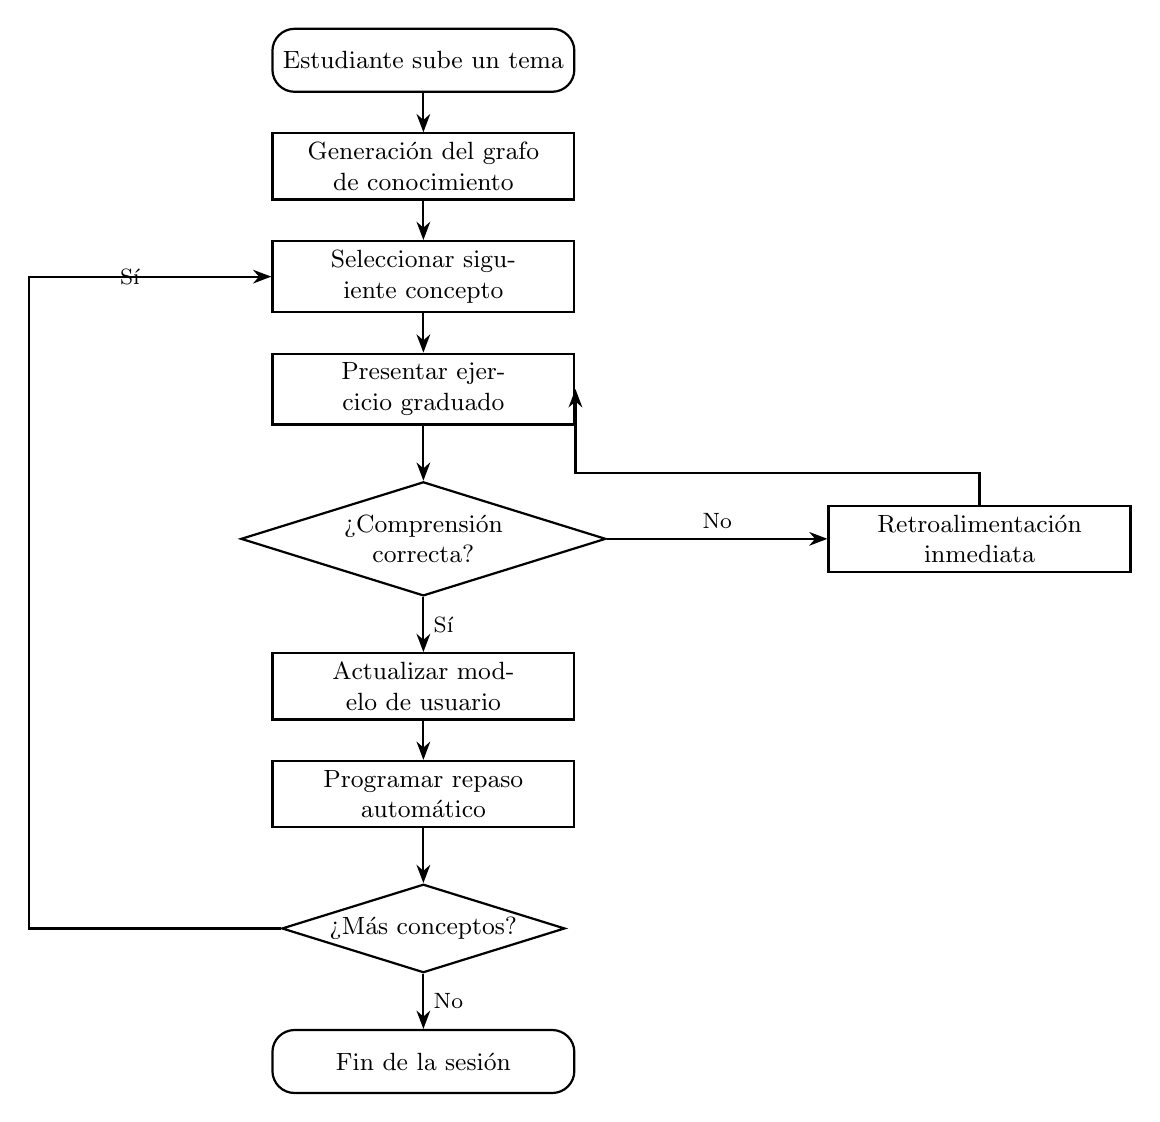
\begin{tikzpicture}[
  node distance=0.5cm,
  startstop/.style={rectangle, rounded corners=8pt, draw, thick,
                    text width=3.6cm, minimum height=0.8cm,
                    align=center, font=\small},
  process/.style={rectangle, draw, thick,
                  text width=3.6cm, minimum height=0.8cm,
                  align=center, font=\small},
  decision/.style={diamond, draw, thick, aspect=3.2,
                   text width=2.4cm, align=center,
                   font=\small, inner sep=1pt},
  arr/.style={-{Stealth}, thick},
]
\node[startstop] (start)     {Estudiante sube un tema};
\node[process, below=of start]    (grafo)    {Generación del grafo de conocimiento};
\node[process, below=of grafo]    (select)   {Seleccionar siguiente concepto};
\node[process, below=of select]   (ejercicio){Presentar ejercicio graduado};
\node[decision, below=0.7cm of ejercicio] (correcto) {¿Comprensión correcta?};
\node[process, right=2.8cm of correcto]  (feedback) {Retroalimentación\\ inmediata};
\node[process, below=0.7cm of correcto]  (actualizar){Actualizar modelo de usuario};
\node[process, below=of actualizar]      (espaciado) {Programar repaso automático};
\node[decision, below=0.7cm of espaciado](mas)       {¿Más conceptos?};
\node[startstop, below=0.7cm of mas]     (end)       {Fin de la sesión};
% Flujo principal
\draw[arr] (start)     -- (grafo);
\draw[arr] (grafo)     -- (select);
\draw[arr] (select)    -- (ejercicio);
\draw[arr] (ejercicio) -- (correcto);
\draw[arr] (correcto)  -- node[right, font=\footnotesize]{Sí} (actualizar);
\draw[arr] (correcto.east) -- node[above, font=\footnotesize]{No} (feedback.west);
\draw[arr] (feedback.north) -- ++(0,0.4) -| (ejercicio.east);
\draw[arr] (actualizar) -- (espaciado);
\draw[arr] (espaciado)  -- (mas);
\draw[arr] (mas)        -- node[right, font=\footnotesize]{No} (end);
% Bucle: siguiente concepto
\draw[arr] (mas.west) -- ++(-3.2,0) |- node[left, font=\footnotesize, near end]{Sí} (select.west);
\end{tikzpicture}
\caption{Flujo del proceso de estudio adaptativo en la plataforma.}
\fuente{Elaboración propia, 2026.}
\end{figure}

% =============================================================================
% 7. DISEÑO METODOLÓGICO
% =============================================================================
\section{Diseño Metodológico}

El proyecto sigue una metodología de desarrollo incremental por fases, donde cada fase entrega un módulo funcional que se integra con los anteriores. La validación es técnica: se verifica que el sistema produce los comportamientos diseñados de manera consistente.

\subsection{Tipo de Investigación}

La investigación es aplicada. Se toma conocimiento existente de las ciencias cognitivas y la ingeniería de software y se aplica al diseño y construcción de un sistema funcional que resuelve un problema real e identificable. El enfoque es mixto: cuantitativo en la medición del comportamiento del sistema (tiempos de respuesta, tasas de error, precisión del motor de dificultad y del algoritmo de espaciado) y cualitativo en la validación de la experiencia del usuario (comprensión del flujo, usabilidad de la interfaz y percepción del acompañamiento adaptativo).

\subsection{Método de Investigación}

Se utiliza el método de desarrollo iterativo incremental. El sistema se construye en fases comenzando por los módulos centrales: el grafo de conocimiento y el modelo de usuario. Cada fase integra un nuevo módulo, se prueba su funcionamiento de forma aislada y luego su integración con los módulos anteriores. Las decisiones de diseño se toman basándose en evidencia de la literatura de ciencias cognitivas y en los resultados de las pruebas de cada fase.

\subsection{Técnicas e Instrumentos de Investigación}

\subsubsection{Técnicas}

Se utilizan pruebas funcionales por módulo para verificar que cada componente produce el comportamiento esperado. Se aplican entrevistas y encuestas con estudiantes de último año para validar la usabilidad y pertinencia del flujo. Se realiza revisión de literatura científica en ciencias cognitivas como base para las decisiones de diseño del motor de dificultad y el algoritmo de espaciado. Se efectúa análisis comparativo de plataformas existentes para documentar las brechas que el sistema resuelve.

\subsubsection{Instrumentos}

Los instrumentos correspondientes a cada técnica son los siguientes: guías de entrevista semiestructurada y cuestionarios de usabilidad para la validación con usuarios; fichas de revisión bibliográfica para la sistematización de la literatura científica; y matrices de análisis comparativo para la evaluación de plataformas existentes.

\subsection{Población y Muestra}

La población objetivo son los estudiantes de último año de colegio en Santa Cruz de la Sierra. Las fuentes primarias son los estudiantes de último año del Colegio Cardenal Cushing, consultados mediante entrevistas y pruebas de usabilidad. Las fuentes secundarias incluyen literatura científica en ciencias cognitivas, documentación técnica de las tecnologías utilizadas y análisis de plataformas educativas existentes como Khan Academy, Duolingo y Anki. La muestra para la validación se selecciona mediante muestreo no probabilístico por conveniencia, dado el carácter aplicado de la investigación.

% =============================================================================
% 8. ÍNDICE TENTATIVO
% =============================================================================
\section{Índice Tentativo}

\begin{indicetentativo}
INTRODUCCIÓN \\[2pt]
CAPÍTULO I. MARCO GENERAL \\
\quad 1.1 Antecedentes \\
\quad 1.2 Planteamiento del Problema \\
\quad\quad 1.2.1 Formulación del Problema \\
\quad\quad 1.2.2 Árbol del Problema \\
\quad 1.3 Objetivos \\
\quad\quad 1.3.1 Objetivo General \\
\quad\quad 1.3.2 Objetivos Específicos \\
\quad 1.4 Justificación \\
\quad\quad 1.4.1 Justificación Técnica \\
\quad\quad 1.4.2 Justificación Económica \\
\quad\quad 1.4.3 Justificación Social \\
\quad 1.5 Metodología \\
\quad\quad 1.5.1 Enfoque de la Investigación \\
\quad\quad 1.5.2 Tipo de Investigación \\
\quad\quad 1.5.3 Método de Investigación \\
\quad\quad 1.5.4 Técnicas e Instrumentos de Investigación \\
\quad\quad 1.5.5 Fuentes de Información \\
\quad\quad 1.5.6 Propuesta \\[2pt]
CAPÍTULO II. MARCO TEÓRICO Y TECNOLÓGICO \\
\quad 2.1 Fundamentos de Ingeniería de Software \\
\quad\quad 2.1.1 Metodologías de Desarrollo de Software \\
\quad\quad 2.1.2 Modelo Seleccionado \\
\quad 2.2 Análisis de Requerimientos y Modelado \\
\quad\quad 2.2.1 Requerimientos Funcionales y No Funcionales \\
\quad\quad 2.2.2 Técnicas para Levantamiento y Análisis \\
\quad\quad 2.2.3 Modelado de Sistemas con UML \\
\quad\quad 2.2.4 Modelo C4 de Arquitectura de Software \\
\quad 2.3 Arquitectura de Sistemas \\
\quad\quad 2.3.1 Modelo Cliente-Servidor \\
\quad\quad 2.3.2 Arquitecturas en Aplicaciones Web \\
\quad 2.4 Tecnologías de Desarrollo \\
\quad\quad 2.4.1 Backend: Lenguajes, Frameworks y Estilos de API \\
\quad\quad 2.4.2 Frontend: Frameworks, Componentes y Renderizado \\
\quad\quad 2.4.3 Bases de Datos y Persistencia de Datos \\
\quad\quad 2.4.4 Infraestructura, Despliegue y Contenedores \\
\quad 2.5 Experiencia de Usuario y Accesibilidad \\
\quad\quad 2.5.1 Diseño Centrado en el Usuario (UCD) \\
\quad\quad 2.5.2 Principios Básicos de UX en Aplicaciones Web \\
\quad\quad 2.5.3 Accesibilidad Web y Buenas Prácticas \\[2pt]
CAPÍTULO III. ANÁLISIS Y DISEÑO DEL SISTEMA PROPUESTO \\
\quad 3.1 Análisis del Contexto Operativo \\
\quad 3.2 Definición de Requerimientos del Sistema \\
\quad 3.3 Modelo de Procesos y Flujo de Trabajo \\
\quad 3.4 Diseño de la Arquitectura de la Solución \\
\quad 3.5 Diseño de Datos \\
\quad 3.6 Diseño de la Interacción Usuario-Sistema \\
\quad 3.7 Seguridad y Cumplimiento \\
\quad 3.8 Plan de Desarrollo por Incrementos o Iteraciones \\[2pt]
CAPÍTULO IV. CONSTRUCCIÓN E IMPLEMENTACIÓN DEL SISTEMA \\
\quad 4.1 Ambiente de Desarrollo e Implementación \\
\quad 4.2 Desarrollo por Incrementos \\
\quad 4.3 Integración y Despliegue del Sistema \\
\quad 4.4 Manual Técnico \\
\quad 4.5 Manual de Usuario \\[2pt]
CONCLUSIONES \\
RECOMENDACIONES \\
REFERENCIAS BIBLIOGRÁFICAS \\
ANEXOS
\end{indicetentativo}

% =============================================================================
% 9. MARCO TEÓRICO
% =============================================================================
\section{Marco Teórico}

Los fundamentos teóricos del presente trabajo se organizan en cuatro áreas: ciencias cognitivas, aprendizaje adaptativo, grafos de conocimiento e ingeniería de software. Estas áreas permiten explicar por qué el sistema debe personalizar el proceso de estudio, cómo puede representar el conocimiento y bajo qué enfoque técnico se construirá la plataforma.

\subsection{Procesamiento de la información, memoria y retención}

El modelo de procesamiento de la información plantea que la memoria humana opera mediante etapas sucesivas de registro sensorial, memoria a corto plazo y memoria a largo plazo \parencite{atkinson1968}. Desde este enfoque, estudiar no consiste únicamente en exponerse al contenido, sino en procesarlo activamente, recuperarlo y revisarlo en momentos adecuados. La curva del olvido descrita por \textcite{ebbinghaus1913} muestra que la retención disminuye con el tiempo si no existen repasos posteriores, mientras que la práctica distribuida mejora el recuerdo frente a sesiones concentradas \parencite{cepeda2006}. Por ello, el sistema propuesto incorpora repasos automáticos y evita que el estudiante avance sin consolidar conceptos previos.

\begin{figure}[H]
\centering
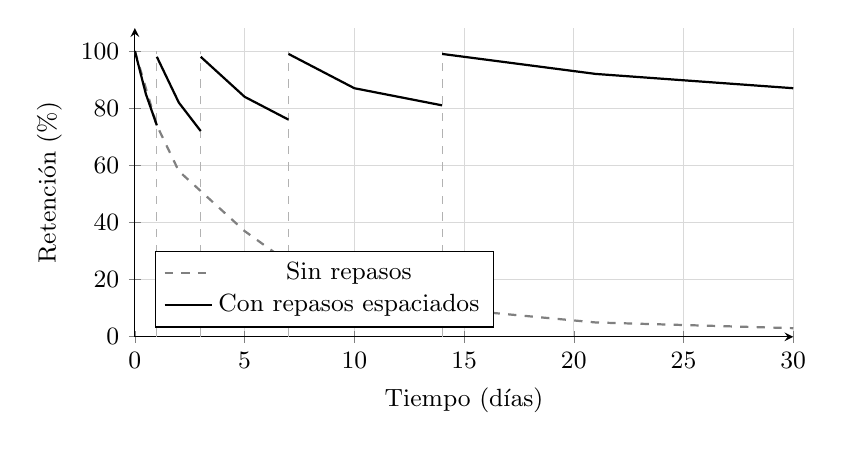
\begin{tikzpicture}
\begin{axis}[
  width=0.82\textwidth,
  height=5.5cm,
  xlabel={Tiempo (días)},
  ylabel={Retención (\%)},
  xmin=0, xmax=30,
  ymin=0, ymax=108,
  xtick={0,5,10,15,20,25,30},
  ytick={0,20,40,60,80,100},
  legend pos=south west,
  legend style={font=\small},
  grid=major,
  grid style={line width=0.3pt, draw=gray!30},
  axis lines=left,
  label style={font=\small},
  tick label style={font=\small},
]
% Líneas verticales en los puntos de repaso
\addplot[gray!60, thin, dashed, forget plot] coordinates {(1,0)(1,100)};
\addplot[gray!60, thin, dashed, forget plot] coordinates {(3,0)(3,100)};
\addplot[gray!60, thin, dashed, forget plot] coordinates {(7,0)(7,100)};
\addplot[gray!60, thin, dashed, forget plot] coordinates {(14,0)(14,100)};
% Sin repasos — caída exponencial aproximada
\addplot[thick, gray, dashed] coordinates {
  (0,100)(1,74)(2,58)(3,51)(5,37)(7,26)(10,17)(14,10)(21,5)(30,3)
};
\addlegendentry{Sin repasos}
% Con repasos espaciados — patrón de dientes de sierra con valles crecientes
\addplot[thick, black] coordinates {(0,100)(0.5,85)(1,74)};
\addlegendentry{Con repasos espaciados}
\addplot[thick, black, forget plot] coordinates {(1,98)(2,82)(3,72)};
\addplot[thick, black, forget plot] coordinates {(3,98)(5,84)(7,76)};
\addplot[thick, black, forget plot] coordinates {(7,99)(10,87)(14,81)};
\addplot[thick, black, forget plot] coordinates {(14,99)(21,92)(30,87)};
\end{axis}
\end{tikzpicture}
\caption{Curva del olvido de Ebbinghaus: retención sin repasos y con repasos espaciados. Las líneas verticales punteadas indican los momentos de repaso.}
\fuente{Adaptado de \textcite{ebbinghaus1913} y \textcite{cepeda2006}.}
\end{figure}

La verificación activa de comprensión también es relevante. \textcite{roediger2006} muestran que recuperar información mediante pruebas fortalece la retención más que releer pasivamente. Además, la carga cognitiva debe controlarse para no saturar al estudiante durante la resolución de tareas \parencite{sweller1988}. Estos fundamentos justifican el uso de ejercicios graduados, retroalimentación inmediata y control progresivo de dificultad.

\subsection{Aprendizaje adaptativo y modelos de usuario}

El aprendizaje adaptativo busca ajustar el contenido, el ritmo y la dificultad a las características del estudiante. \textcite{bloom1984} demostró la ventaja del acompañamiento individual frente a la instrucción grupal, lo que respalda la necesidad de sistemas que aproximen una experiencia personalizada. En la misma línea, los sistemas tutores inteligentes han mostrado resultados relevantes cuando modelan el estado del estudiante y entregan apoyo durante la resolución de tareas \parencite{vanlehn2011}.

Para personalizar el aprendizaje es necesario representar el conocimiento actual del usuario. El seguimiento de conocimiento permite estimar qué conceptos domina el estudiante y cuáles requieren refuerzo \parencite{corbett1994}. Los modelos de usuario en sistemas educativos adaptativos amplían esta idea al registrar desempeño, progreso, preferencias y necesidades individuales \parencite{brusilovsky2007}. En el presente proyecto, este fundamento se traduce en un modelo de usuario que registra el estado de cada concepto y guía la selección del contenido siguiente.

\subsection{Grafos de conocimiento aplicados a educación}

Un grafo de conocimiento representa entidades y relaciones mediante nodos y enlaces, permitiendo organizar información compleja de forma explícita \parencite{hogan2021}. En educación, esta estructura permite modelar conceptos, prerrequisitos y dependencias entre temas. De esta manera, el sistema puede determinar qué debe estudiar primero un usuario y qué conceptos se ven afectados cuando falla una respuesta.

Los grafos de conocimiento educativos han sido utilizados para estructurar dominios de aprendizaje y apoyar sistemas de recomendación o rutas personalizadas \parencite{chen2018}. En este proyecto, el grafo cumple una función central: organizar el currículo de matemáticas de último año según sus relaciones de prerrequisito, establecer las dependencias entre conceptos y alimentar el modelo de dificultad, comprensión y repaso.

\subsection{Ingeniería de software y desarrollo de la plataforma}

Desde la ingeniería de software, el proyecto requiere un proceso de desarrollo controlado que permita construir módulos verificables e integrarlos progresivamente. \textcite{sommerville2016} plantea que el desarrollo de software debe partir de requerimientos claros, diseño, implementación, pruebas y evolución. \textcite{pressman2014} destaca la importancia de dividir sistemas complejos en componentes y validar cada incremento antes de avanzar.

Por esta razón, la plataforma se plantea como una solución construida por fases: grafo de conocimiento, modelo de usuario, motor de dificultad, algoritmo de espaciado, retroalimentación e integración final. Este enfoque permite reducir el riesgo técnico, validar cada módulo y mantener la trazabilidad entre el problema educativo y la solución implementada.

% =============================================================================
% 10. CRONOGRAMA
% =============================================================================
\section{Cronograma}

El desarrollo del proyecto se organiza en cuatro fases incrementales durante la gestión 2026, en el período comprendido entre abril y diciembre. Cada fase entrega un módulo funcional validado que se integra con los anteriores.

\begin{table}[H]
\centering
\caption{Cronograma de desarrollo por fases — gestión 2026.}
\begin{tabular}{llll}
\toprule
\textbf{Fase} & \textbf{Actividad} & \textbf{Inicio} & \textbf{Fin} \\
\midrule
1 & Grafo de conocimiento y modelo de usuario & Abril & Mayo \\
2 & Motor de dificultad progresiva & Junio & Julio \\
3 & Algoritmo de espaciado y retroalimentación & Agosto & Septiembre \\
4 & Integración, pruebas y validación con usuarios & Octubre & Diciembre \\
\bottomrule
\end{tabular}
\fuente{Elaboración propia, 2026.}
\end{table}

% =============================================================================
% 11. REFERENCIAS BIBLIOGRÁFICAS
% =============================================================================
\referencias

% =============================================================================
% ANEXOS
% =============================================================================
\seccioncuerpo{ANEXOS}

\end{document}
